\documentclass[12pt,a4paper]{report}
\usepackage[a4paper,
    left=1.25in,
    right=1in,
    top=1in,
    bottom=1in]{geometry} % Required for inserting images
\usepackage{fullpage}
\usepackage{mathptmx}
\usepackage{titletoc}
\usepackage[titles]{tocloft}
\usepackage{booktabs}   % For professional table formatting
\usepackage{array}      % For enhanced table control
\usepackage{siunitx}    % For proper number formatting
%\usepackage{geometry}   % To adjust page margins
\usepackage{float}
\usepackage{tikz}
\usetikzlibrary{shapes.geometric,calc, arrows.meta, positioning}
\usepackage{amsmath}
\usepackage{lipsum}
\usepackage{acronym}
\usepackage{graphicx}
\graphicspath{ {./images/} }
\usepackage{hyperref}
\usepackage[utf8]{inputenc}
\usepackage{fancyhdr}
%\usepackage{fontspec}
\usepackage{pgfgantt}
\usepackage{xcolor}

\usepackage[labelfont=bf, font=bf, justification=centering, font=small]{caption}
\captionsetup[figure]{labelfont=bf, font=bf, justification=centering, font=small, labelsep=period}
\captionsetup[table]{labelfont=bf, font=bf, justification=centering, font=small, labelsep=period, position=above}
  
% Line spacing
\usepackage{setspace}
\onehalfspacing  % or use \singlespacing or \doublespacing as needed

% Paragraph spacing
\setlength{\parskip}{0.75em}  % space between paragraphs
\setlength{\parindent}{0pt}   % no indentation (you already have this)

% Custom font sizes for headings
\usepackage{sectsty} % to customize section font sizes

% Normal text font size is already 12pt (from documentclass)

% Normal heading style (like \textbf 12pt) - redefine \normalfont
\renewcommand\normalsize{\fontsize{12}{14}\selectfont} % 12pt font with 14pt baseline skip

% Section headings (14pt)
\sectionfont{\fontsize{14}{16}\selectfont\bfseries} 

% Subsection headings (optional, keep smaller)
\subsectionfont{\fontsize{12}{14}\selectfont\bfseries}

% Chapter (main heading) size (16pt bold centered)
\usepackage{titlesec}
\titleformat{\chapter}[display]
  {\normalfont\bfseries\fontsize{16}{18}\selectfont\centering}
  {\chaptername\ \thechapter}{1em}{}

\renewcommand*\contentsname{Table of Contents}

% Redefine the \numberline command for figures
\newlength{\mylen}
\renewcommand{\cftdotsep}{0.5}
\renewcommand{\cftfigpresnum}{\hspace*{-1.5em}\figurename\enspace}
\renewcommand{\cftfigaftersnum}{:}
\settowidth{\mylen}{\cftfigpresnum\cftfigaftersnum}
\addtolength{\cftfignumwidth}{\mylen}


\renewcommand{\cftdotsep}{0.5}
\renewcommand{\cfttabpresnum}{\hspace*{-1.5em}\tablename\enspace}
\renewcommand{\cfttabaftersnum}{:}
\settowidth{\mylen}{\cfttabpresnum\cfttabaftersnum}
\addtolength{\cfttabnumwidth}{\mylen}


\titlecontents{chapter}
[5.5em] %5.3
{\smallskip}
{\contentslabel[\bfseries{\chaptername}~\thecontentslabel{:}]{5.5em}\textbf}%\thecontentslabel
{\hspace*{-5.5em}\textbf}% unnumbered chapters
{\titlerule*[0.35pc]{.}\contentspage}[\smallskip]%

\titlecontents{section}
[1.5em] % i
{\smallskip}
{\thecontentslabel\enspace}%\thecontentslabel
{\hspace*{-5.5em}}
{\titlerule*[0.35pc]{.}\contentspage}%]

\titlecontents{subsection}
[7.12em] %
{\smallskip}
{\thecontentslabel\enspace}%\thecontentslabel
{\hspace*{7.12em}}
{\titlerule*[0.35pc]{.}\contentspage}

\makeatletter
\renewcommand{\@makechapterhead}[1]{%\vspace*{50 pt}%
{\setlength{\parindent}{0pt}\normalfont
\bfseries\Huge\chaptername{\hspace*{0.25em}}\centering\thechapter{:}\ #1
\par\nobreak\vspace{16 pt}}}
\makeatother

\makeatletter
\renewcommand{\@makeschapterhead}[1]{%\vspace*{50 pt}%
{\setlength{\parindent}{0pt}\normalfont
\bfseries\Huge\centering\ #1
\par\nobreak\vspace{16 pt}}}
\makeatother
%\renewcommand{\refname}{References} % For article class
\renewcommand{\bibname}{References} % For report/book class

\title{Major}
\author{Sandip Adhikari}
\date{May 2025}

\setlength{\parindent}{0pt}

\begin{document}
\begin{titlepage}
    \thispagestyle{empty}
    \begin{center}
    
    \vspace*{\fill} % * makes latex to not ignore the command
    \vspace*{-1cm}
    {\Large \textbf{TRIBHUVAN UNIVERSITY
}\par}
{\large \textbf{INSTITUTE OF ENGINEERING
}\par}
\vspace{12pt}
KATHMANDU ENGINEERING COLLEGE

KALIMATI, KATHMANDU
\vspace{24pt}

\begin{figure}[ht]
    \centering
    
\includegraphics[scale=0.45]{images/kec.png}
\end{figure}
\vspace{24pt}
{Major Project Proposal Report on\par}
\vspace{6pt}
{\textbf{GARUD-UAV: Land Use Classification Using Deep Learning on Upscaled UAV Images}\par}

\vspace{18pt}
{\textbf{BY}\par}
\vspace{10pt}
    
{POSHAN ACHARYA- KAT078BEI012\par}
{PRANEESHAA DHAKAL- KAT078BEI013\par}
{SANDIP ADHIKARI- KAT078BEI019\par}

\vspace{28pt}
{\textbf{TO}\par}
\vspace{10pt}
{DEPARTMENT OF ELECTRONICS, COMMUNICATION AND INFORMATION ENGINEERING\par}
{KATHMANDU, NEPAL\par}
\vspace{14pt}
{May, 2025\par}

    \vspace*{\fill}

    \end{center}
\end{titlepage}

\pagenumbering{roman}

\chapter*{Acknowledgement}
\addcontentsline{toc}{chapter}{Acknowledgement}
\label{acknowledgement}
We express our gratitude to our project supervisors, \textbf{Er. Sarina Barahi Sthapit} and \textbf{Er. Puspha Dhamala} along with our project coordinator\textbf{ Er. Sujan Shrestha} for providing invaluable support and guidance throughout the project. We are deeply thankful to the Department of Electronics, Communication, and Information Engineering at Kathmandu Engineering College for granting us the opportunity to complete our major project as a part of our syllabus. We wholeheartedly appreciate the esteemed Head of the Department of Electronics, Communication, and Information Engineering, \textbf{Asso. Prof. Er. Suramya Sharma Dahal}. We sincerely appreciate the encouragement, support, constructive criticism, and guidance provided by the entire teaching staff at the Department of Electronics, Communication, and Information Engineering.

%\chapter*{Abstract}
%\addcontentsline{toc}{chapter}{Abstract}
%\label{abstract}
%\lipsum[2-4]

\tableofcontents
\thispagestyle{empty}
\addtocounter{page}{-1}
\newpage

\listoffigures
\addcontentsline{toc}{chapter}{List of Figures}
\newpage

\listoftables
\addcontentsline{toc}{chapter}{List of Tables}
\newpage

\chapter*{List of Abbreviation}
\addcontentsline{toc}{chapter}{List of Abbreviation}
\label{abbreviation}
\begin{acronym}
 \acro{AI}{Artificial Intelligence}
 \acro{GPIO}{General Purpose Input Output}
 \acro{IoT}{Internet of Things}
 \acro{ML}{Machine Learning}
 \acro{RAM}{Random Access Memory}
 \acro{OS}{Operating System}
 \acro{BRNN}{Bidirectional Recurrent Neural Networks}
 \acro{GRU}{Gated Recurrent Units}
 \acro{MIMO}{Multiple Input Multiple Output}
 \acro{SoC}{System-on-Chip}
 \acro{USB}{Universal Serial Bus}
 \acro{Wi-Fi}{Wireless Fidelity}
 \acro{NLP}{Natural Language Processing}
 \acro{TTS}{Text-To-Speech}
 \acro{API}{Application Programming Interface}
 \acro{ARM}{Advanced RISC Machine}
 \acro{RISC}{Reduced Instruction Set Computer}
 \acro{IP}{Internet Protocol}
 \acro{MCU}{Micro-Controller Unit}
\end{acronym}
\newpage

\pagenumbering{arabic}

\chapter{Introduction}
\label{introduction}
\section{Background Theory}
The rapid advancement of Unmanned Aerial Vehicles (UAVs) has transformed applications in environmental monitoring, agriculture, and urban planning by providing cost-effective and high-resolution data collection capabilities \cite{aabid2022reviews} \cite{baballe2022review}. Fixed-wing UAVs, in particular, offer significant advantages for land use image classification due to their extended range, longer endurance, and ability to cover large areas efficiently, making them ideal for wide-areas surveillance and mapping tasks \cite{aabid2022reviews}. These vehicles can capture high-resolution aerial imagery, enabling precise analysis of land use patterns critical for precision agriculture, urban development, and disaster management \cite{baballe2022review} \cite{shakhatreh2019survey}. However, challenges such as limited payload capacity, regulatory constraints, and the need for advanced image processing to achieve high-quality outputs persist, necessitating innovative design and algorithmic solutions \cite{aabid2022reviews}\cite{baballe2022review} .

A key component of this project is the integration of Enhanced Super-Resolution Generative Adversarial Network (ESRGAN), a state-of-the-art deep learning model for single image super-resolution (SISR) introduced by Wang et al. in 2018 \cite{wang2018esrgan}. ESRGAN employs a Generative Adversarial Network (GAN) framework, comprising a generator that creates high-resolution images from low-resolution inputs and a discriminator that ensures realism. Noted for its ability to reconstruct realistic textures and fine details, ESRGAN is ideal for enhancing images captured by UAV-mounted cameras, such as those using Raspberry Pi modules, typically upscaling images by a factor of 4x \cite{wang2018esrgan}. This capability is particularly valuable for land use classification, where high-resolution imagery is essential for identifying intricate land features.

This research project aims to design and develop a fixed-wing UAV tailored for land use image classification, leveraging lightweight materials, advanced sensors, and ESRGAN for enhanced image processing to improve data accuracy and operational efficiency. By addressing design considerations such as aerodynamic efficiency, flight stability, and integration of high-resolution imaging systems, this project seeks to create a UAV capable of collecting and processing aerial imagery for accurate land use analysis \cite{aabid2022reviews}\cite{baballe2022review} . Drawing on prior research, including deep learning applications for UAV systems and their use in precision agriculture \cite{baballe2022review}, this project will optimize UAV performance for environmental monitoring tasks. The outcome is expected to contribute to UAV-based remote sensing, offering a scalable solution for land use analysis in diverse geographical contexts.

\section{Problem Statement}
Land use and land cover (LULC) classification is critical for effective environmental management, agricultural monitoring, urban planning, and disaster response. Traditionally, satellite imagery has been the primary source for such analysis; however, limitations such as low spatial resolution, infrequent data updates, atmospheric disturbances, and high operational costs restrict its applicability for high-precision, real-time monitoring \cite{baballe2022review}. In contrast, UAVs offer a flexible, cost-effective, and scalable solution for high-resolution remote sensing. Among UAV types, fixed-wing aircraft present superior advantages for surveying large geographical areas due to their extended flight duration, aerodynamic efficiency, and higher operational altitudes \cite{aabid2022reviews}\cite{baballe2022review} .

Despite their potential, existing UAV platforms used for LULC classification are often either commercially expensive, overly complex for academic research and field adaptation, or designed around rotary-wing systems that lack the range and endurance needed for broad-area coverage \cite{rotary}. Moreover, there is a lack of integrated, low-cost fixed-wing UAV solutions that combine autonomous navigation, high-resolution image acquisition, and onboard or post-processed land classification capability tailored to specific regional or environmental needs.

Therefore, there exists a critical need to develop a custom-built, fixed-wing UAV system optimized for land use image classification—one that is affordable, reliable, and capable of autonomous operation in varied field conditions. This research project addresses that need by designing and implementing a fixed-wing UAV equipped with geo-referenced imaging systems and an image-processing pipeline to enable accurate and efficient land use classification.

\section{Objectives}

\begin{enumerate}
    \item To design and build a fixed-wing UAV equipped with a lightweight camera system capable of capturing aerial image.
    \item To improve the quality of captured aerial images through image upscaling techniques for enhanced clarity and detail.
    \item To perform deep learning based land use classification using the upscaled high-resolution aerial imagery.
\end{enumerate}



\chapter{Literature Review}
\label{literaturereview}
The rapid development of Unmanned Aerial Vehicles (UAVs) has significantly impacted remote sensing, particularly in Land Use and Land Cover (LULC) classification. UAVs can capture high-resolution imagery, which is ideal for extracting fine-grained spatial details. However, challenges such as varying resolution, atmospheric distortion, and inconsistent lighting can affect the quality of the images. The application of deep learning techniques, particularly convolutional neural networks (CNNs), in enhancing UAV imagery via image upscaling is a promising direction, as seen in the proposed Gaurad-UAV model.

High-resolution data is crucial for accurate land use classification. Traditional satellite-based imagery often suffers from resolution constraints and longer revisit times. UAVs overcome these issues by offering greater spatial resolution and flexible data acquisition. Studies such as [6] and [7] have successfully demonstrated the use of UAV imagery for detailed classification of urban and agricultural landscapes. In [6], Bui et al. employed a CNN model combined with UAV images and digital surface models (DSMs) to achieve a high overall classification accuracy of over 91% in urban mapping tasks.

Deep learning models, especially transfer learning-based CNNs, have proven highly effective for LULC classification. Naushad et al. [7] used models like VGG16 and Wide Residual Networks (WRNs) to classify complex land use categories with an accuracy exceeding 98%, highlighting the capability of deep features to capture subtle variations in land cover types.

Image upscaling, or single-image super-resolution (SISR), has emerged as a key pre-processing step to improve classification performance. Tuna et al. [8] applied CNN-based super-resolution methods to remote sensing images, showing improved visual quality and feature detectability, which in turn enhanced classification outcomes. This process helps generate higher-resolution approximations of low-resolution images, mitigating the effects of noise and data sparsity in UAV captures.

The Gaurad-UAV framework is proposed as a comprehensive approach that leverages deep CNNs for image upscaling before land use classification. While specific architectural and experimental details are yet to be broadly published, the conceptual foundation aligns well with existing literature. By enhancing image resolution, Gaurad-UAV aims to improve the feature quality available to classification models, thereby increasing accuracy and robustness in heterogeneous environments.

In summary, the integration of UAV imagery with deep learning and image super-resolution techniques presents a strong foundation for enhanced LULC classification. Gaurad-UAV, as a deep learning-powered image enhancement pipeline, contributes meaningfully to this domain by addressing the challenge of limited image resolution in high-precision mapping applications.

\chapter{Related Theory}
\label{relatedtheory}
\section{Hardware}
\lipsum[4-8]
\begin{figure}
\centering
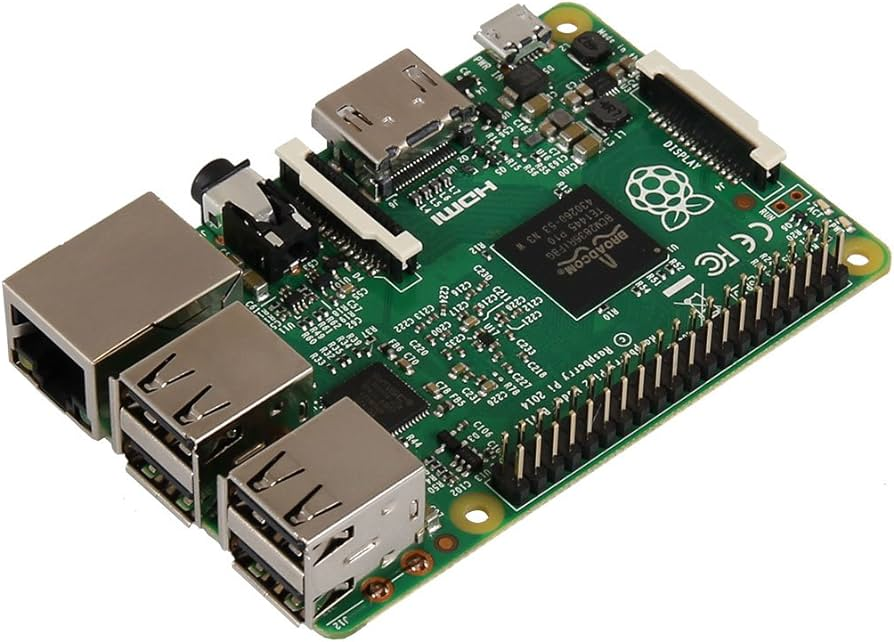
\includegraphics[width=0.5\textwidth]{images/raspimg.jpg}
\caption{Raspberry Pi 4 Model B}

\end{figure}

\section{Software Overview}

\subsection{ESRGAN for Image Super-Resolution}
\begin{figure}[H]
    \centering
    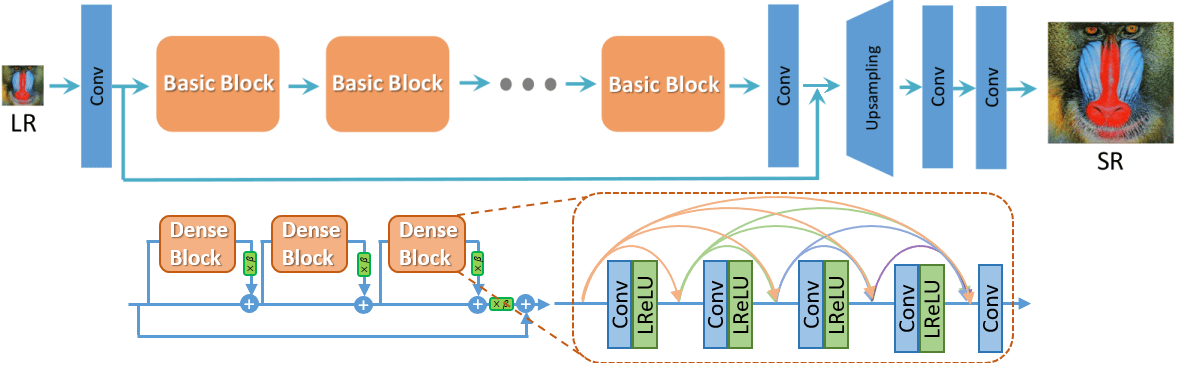
\includegraphics[width=0.85\linewidth]{images/esrganarchi.png}
    \caption{ESRGAN Architecture with Residual-in-Residual Dense Blocks (RRDB)}
    \label{fig:esrgan}
\end{figure}
ESRGAN introduced by Wang \emph{et al.} in 2018 [1], improves upon SRGAN by employing a deep generator built from Residual‑in‑Residual Dense Blocks (RRDB) without batch normalization. Each RRDB combines multiple convolutional layers, local dense connections, and global residual links to capture complex image features. The generator upsamples low‑resolution inputs (e.g.\ 820×616 pixels) by a factor of 4× to high‑resolution outputs (e.g.\ 3280×2464 pixels). The discriminator is relativistic, estimating the probability that a real image is more realistic than a generated one, which enhances stability and visual fidelity. ESRGAN further integrates a perceptual loss based on high‑level VGG features computed before ReLU activations, preserving fine textures and brightness consistency. This design enables ESRGAN to produce photorealistic details, as demonstrated by its victory in the PIRM2018 SR Challenge [1].

In our UAV system, images captured onboard with a Raspberry Pi USB Camera are retrieved post‑flight. ESRGAN runs on a ground PC to upscale extracted frames, recovering critical details (e.g.\ building outlines, vegetation patterns) necessary for accurate land use classification in the Kathmandu region.

\subsection{Comparison of Super-Resolution Models}
We compare ESRGAN with earlier SR approaches:

\begin{table}[H]
\centering
\renewcommand{\arraystretch}{1.2}
\setlength{\tabcolsep}{6pt}
\begin{tabular}{@{} l l p{3cm} p{3cm} p{3cm} @{}}
    \toprule
    \textbf{Model} & \textbf{Year} & \textbf{Architecture} & \textbf{Strengths} & \textbf{Weaknesses} \\
    \midrule
    SRCNN   & 2014 & 3-layer CNN & Simple, fast & Overly smooth outputs [2] \\
    FSRCNN  & 2016 & CNN + deconv & Efficient, higher PSNR [2] & Limited texture detail \\
    EDSR    & 2017 & Deep ResNet & High PSNR, faster [3] & Less perceptual quality \\
    ESRGAN  & 2018 & GAN + RRDB & Realistic textures, sharp edges [1] & Computationally intensive \\
    \bottomrule
  \end{tabular}
  \caption{Comparison of Super-Resolution Models}
\label{tab:sr_models}
\end{table}


\subsection{Land Use Classification}
Land use classification from UAV imagery entails categorizing pixels or patches into classes such as forest, agriculture, water, and urban. Common approaches include:
\begin{itemize}
  \item \textbf{Convolutional Neural Networks (CNNs)}: End‑to‑end models (e.g.\ U‑Net, ResNet, EfficientNet) that learn spatial hierarchies directly from upscaled images [4].
  \item \textbf{Random Forest (RF)}: Ensemble of decision trees trained on raw pixels or derived indices, robust to overfitting and effective for moderate datasets [2,4].
  \item \textbf{Support Vector Machine (SVM)}: Kernel‑based classifier suitable for moderate‑sized, well‑separated classes [2,4].
\end{itemize}
A hybrid approach often combines CNN feature extractors with RF or SVM classifiers, leveraging deep networks for hierarchical feature learning and traditional ML for robust classification when labeled data is limited.

\subsection{Software}
The software pipeline integrates the following tools and libraries:
\begin{itemize}
  \item \textbf{OpenCV}: For image/frame extraction, filtering, and geometric transformations [5].
  \item \textbf{NumPy \& SciPy}: Core numerical and array operations for preprocessing.
  \item \textbf{scikit-learn}: Implements RF and SVM classifiers, data splitting, scaling, and evaluation utilities [6].
  \item \textbf{TensorFlow \& PyTorch}: Deep learning frameworks for ESRGAN and CNN implementation. PyTorch (BasicSR toolkit) eases experimentation [7], while TensorFlow (TF‑Hub ESRGAN) supports scalable deployment [8].
  \item \textbf{GDAL/Rasterio}: For handling geo-referenced imagery and aligning with regional GIS data [9].
\end{itemize} 


\subsection{Dataset}

\textbf{1. Kathmandu Land Use Datasets}

Region-specific datasets used for land use classification in Kathmandu:

\begin{itemize}
  \item \textbf{Nepal National Land Cover Dataset}: Annual land-cover maps (2000–2022) from Landsat imagery via Google Earth Engine, covering forests, agriculture, water, and built-up areas[10].
  \item \textbf{Kathmandu City Land Use Shapefiles}: Urban land use polygons (residential, commercial, parks) for Kathmandu Metropolitan City (2011) from ICIMOD[11].
  \item \textbf{OpenStreetMap Polygons}: Land-use tags for Kathmandu accessible through the Humanitarian Data Exchange[12].
\end{itemize}

\textbf{2. Image Super-Resolution Datasets}

Datasets used to train and evaluate ESRGAN and other super-resolution models:

\begin{itemize}
  \item \textbf{DIV2K}: A large-scale dataset designed for image super-resolution, consisting of 1000 high-resolution images and their corresponding low-resolution counterparts. Suitable for training deep SR models.
  \item \textbf{Set5 and Set14}: Benchmark datasets commonly used for evaluating the performance of super-resolution models. While smaller in size, they are widely adopted for quantitative comparisons.
\end{itemize}

These datasets provide essential ground truth for training and validating both our land use classification pipeline and image super-resolution models.



\chapter{Feasibility Study}
\label{feasiblity}
\section{Technical Feasibility}
\begin{table}[h]
\caption{Hardware Specification Table}
\vspace{12pt}
\centering
\begin{tabular}{|c|c|c|}
\hline
Column 1 & Column 2 & Column 3 \\
\hline
Item 1   & Item 2   & Item 3   \\
Item 4   & Item 5   & Item 6   \\
Item 7   & Item 8   & Item 9   \\
\hline
\end{tabular}

\label{tab:Hardware Specification Table}
\end{table}
\section{Economic Feasibility}
\lipsum[4-8]



\chapter{Methodology}
\label{methodology}
\section{System Block Diagram}

\tikzset{
    block/.style = {
        rectangle, 
        rounded corners, 
        minimum width=3cm, 
        minimum height=1cm, 
        align=center, 
        draw=black, 
        fill=white
    },
    subblock/.style = {
        rectangle, 
        minimum width=1.5cm, 
        minimum height=0.7cm, 
        align=center, 
        draw=black, 
        fill=gray!20
    },
    arrow/.style = {
        thick, 
        -{Stealth[scale=1.2]}
    }
}

\begin{tikzpicture}[node distance=1.2cm]

% UAV System
\node[block, minimum width=7cm, minimum height=3cm] (uav) {UAV};
    \node[subblock] (pi) at ([xshift=0cm, yshift=0cm]uav.north west) {RPi};
    \node[subblock] (camera) at ([xshift=0cm, yshift=0cm]uav.south west) {Camera};
    \node[subblock] (receiver) at ([xshift=0cm, yshift=-1.5cm]uav.north east) {Receiver\\Control};

% Ground System (to the left/west of UAV)
\node[block, right=4cm of uav] (ground) {Ground\\Transmitter};

% Image Upscaling just below Camera
\node[block, below=2cm of uav] (upscale) {Image Upscaling\\(Deep Learning)};

% Land Use Classification below Image Upscaling
\node[block, below=of upscale] (classify) {Land Use\\Classification};
\node[block, below=of classify] (analysis) {Result\\Analysis};

% Data Flow
\begin{scope}[arrow]
    \draw (ground.west) -- (receiver.east); % straight line
    \draw (uav.south) -- node[right, xshift=0.2cm] {Raw\\Images} (upscale.north);
    \draw (upscale) -- (classify);
    \draw (classify) -- (analysis);
\end{scope}

% Legend

\node[align=center] at ($(analysis.south) + (0,-1)$) 
    {\footnotesize \textbf{Figure~\thefigure: System Block Diagram of UAV System}};

\end{tikzpicture}
 
\subsection{System Description}

The system consists of a fixed-wing UAV platform equipped with essential components for flight and data collection. The UAV includes:

\begin{itemize}
    \item \textbf{ESC (Electronic Speed Controller):} Regulates the speed of the motor driving the propeller.
    \item \textbf{Propeller:} Provides thrust for UAV flight.
    \item \textbf{4 Servos:} Control the movement of aerodynamic surfaces like ailerons, elevator, and rudder for flight maneuverability.
    \item \textbf{Battery:} Powers the entire onboard system.
    \item \textbf{UAV Receiver:} Receives control signals from the ground-based transmitter.
    \item \textbf{Raspberry Pi + Camera Module:} Captures aerial images during flight.
\end{itemize}

The ground transmitter sends flight control commands to the UAV receiver. The Raspberry Pi processes input from the onboard camera and stores captured images.

These images are then passed to the image upscaling module using deep learning methods, enhancing the resolution and clarity. The upscaled images are further processed through a classification model to identify land use categories.

Finally, the results from the classification are analyzed for insights, contributing to high-resolution land use mapping from UAV-acquired data.


\chapter{Expected Output}
\label{result}
\section{Expected Output}
\lipsum[4-8]

\chapter*{Gantt Chart}
\addcontentsline{toc}{chapter}{Gantt Chart}
\label{ganttchart}
\begin{figure}[ht]
    \centering
    
\includegraphics[scale=0.45]{images/kec.png}
\end{figure}

\chapter*{Cost Estimation}
\addcontentsline{toc}{chapter}{Cost Estimation}
\label{cost estimation}

% Table 1: Electronics & Core Components
\section*{Electronics \& Core Components}
\begin{table}[h]
\centering
\caption{Electronics and Core Components for Fixed-Wing UAV}
\begin{tabular}{l c S[table-format=5.0]}
\toprule
\textbf{Item} & \textbf{Quantity} & \textbf{Cost (NRs)} \\
\midrule
FLYSKY Receiver & 1 & 8000 \\
30A ESC Skywalker & 1 & 2000 \\
Flight Stabilizer (NXE4 EVO) & 1 & 4500 \\
1000KV Brushless Motor & 1 & 800 \\
MG996 Metal Gear Servo & 4 & 3040 \\
2200mAh 3S LiPo Battery & 1 & 3150 \\
Buck Module Voltage Regulator & 1 & 550 \\
Raspberry Pi with USB Camera and HDMI Cable & 1 & {TBD} \\
Raspberry Pi USB Camera and HDMI Cable & 1 & {TBD} \\
\bottomrule
\end{tabular}
\end{table}

% Table 2: Frame & Construction Materials
\section*{Frame \& Construction Materials}
\begin{table}[h]
\centering
\caption{Frame and Construction Materials for Fixed-Wing UAV}
\begin{tabular}{l c S[table-format=5.0]}
\toprule
\textbf{Item} & \textbf{Quantity} & \textbf{Cost (NRs)} \\
\midrule
Depron Sheet & 4 & 10000 \\
Aluminum Motor Mount (L-shape) & 1 & 150 \\
Push Rod (1m) & 2 & 400 \\
\bottomrule
\end{tabular}
\end{table}

% Table 3: Miscellaneous Accessories
\section*{Miscellaneous Accessories}
\begin{table}[h]
\centering
\caption{Miscellaneous Accessories for Fixed-Wing UAV}
\begin{tabular}{l c S[table-format=3.0]}
\toprule
\textbf{Item} & \textbf{Quantity} & \textbf{Cost (NRs)} \\
\midrule
Hot Glue Gun Stick & 10 & 200 \\
Duct/Binding Tape & 3 rolls & 300 \\
XT60 Connector Pair & 2 & 500 \\
3-Pin Orange Connector Pair & 4 & 60 \\
Servo Wire Cable (5m) & 1 & 75 \\
Propeller (7x5 inch) & 4 & 300 \\
Bullet Propeller Holder Adapter & 1 & 170 \\
Jumper Wire (MM, MF, FF, each 5) & 15 & 30 \\
\bottomrule
\end{tabular}
\end{table}


%\chapter*{References}
\addcontentsline{toc}{chapter}{References}
\bibliographystyle{plain} % or another style like ieee, unsrt, etc.
\bibliography{references} % references.bib (no .bib extension)

\end{document}





